

\documentclass[aspectratio=169,11pt]{beamer}

% -----------------------------------------------------------------------------
% Self-contained presentation setup
% -----------------------------------------------------------------------------
\usepackage[T1]{fontenc}
\usepackage{lmodern}
\usepackage{amsmath,amssymb,mathtools}
\usepackage{booktabs}
\usepackage{tabularx}
\usepackage{listings}
\usepackage{tikz}
\usepackage[most]{tcolorbox}
\usepackage{appendixnumberbeamer}
\usetikzlibrary{arrows.meta,calc,decorations.pathreplacing,fit,matrix,positioning,shapes.geometric}

\usetheme{Boadilla}
\usecolortheme{seagull}
\setbeamertemplate{navigation symbols}{}
\setbeamertemplate{items}[circle]
\setbeamertemplate{enumerate items}[default]
\setbeameroption{hide notes}

\definecolor{osblue}{RGB}{28,86,145}
\definecolor{osgreen}{RGB}{36,125,91}
\definecolor{osorange}{RGB}{202,105,36}
\definecolor{osred}{RGB}{166,45,45}
\definecolor{osgray}{RGB}{74,85,104}
\definecolor{ospurple}{RGB}{101,67,135}
\setbeamercolor{structure}{fg=osblue}
\setbeamercolor{alerted text}{fg=osred}
\setbeamercolor{block title}{bg=osblue!15,fg=black}
\setbeamercolor{block body}{bg=osblue!4,fg=black}

\newcommand{\concept}[1]{\textcolor{osblue}{\textbf{#1}}}
\newcommand{\code}[1]{\texttt{#1}}
\newcommand{\smallnote}[1]{\par\vspace{0.2em}{\scriptsize\color{osgray}#1}}
\newcolumntype{C}{>{\centering\arraybackslash}X}
\newcolumntype{L}{>{\raggedright\arraybackslash}X}
\newcommand{\runblock}[4]{%
  \filldraw[fill=#4,draw=white] (#1,.2) rectangle (#2,.9);
  \node at ({(#1+#2)/2},.55) {#3};
}
\newcommand{\runticks}[1]{%
  \foreach \tick in {#1}{\draw (\tick,.08)--(\tick,-.08)
    node[below,font=\scriptsize]{\tick};}
}
\newcommand{\meanresults}[3]{%
  \begin{tcolorbox}[title=Final means (time units; rounded)]
    \centering $\overline{T}=#1\qquad\overline{W}=#2\qquad\overline{R}=#3$
  \end{tcolorbox}
}

\tcbset{
  enhanced,
  boxrule=.7pt,
  arc=1.5mm,
  left=1.2mm,right=1.2mm,top=.8mm,bottom=.8mm,
  colback=osblue!3,
  colframe=osblue!60
}

\lstset{
  basicstyle=\scriptsize\ttfamily,
  keywordstyle=\color{osblue}\bfseries,
  commentstyle=\color{osgreen!80!black},
  stringstyle=\color{osred},
  numbers=left,
  numberstyle=\tiny\color{osgray},
  numbersep=5pt,
  frame=single,
  rulecolor=\color{black!20},
  backgroundcolor=\color{black!2},
  breaklines=true,
  showstringspaces=false,
  columns=fullflexible,
  keepspaces=true
}

\setbeamertemplate{footline}{%
  \leavevmode%
  \hbox{%
    \begin{beamercolorbox}[wd=.18\paperwidth,ht=2.6ex,dp=1.1ex,center]{author in head/foot}
      \insertshortauthor
    \end{beamercolorbox}%
    \begin{beamercolorbox}[wd=.64\paperwidth,ht=2.6ex,dp=1.1ex,center]{title in head/foot}
      \insertshorttitle\ifx\insertsection\empty\else\enspace---\enspace\insertsection\fi
    \end{beamercolorbox}%
    \begin{beamercolorbox}[wd=.18\paperwidth,ht=2.6ex,dp=1.1ex,center]{date in head/foot}
      \insertframenumber{} / \inserttotalframenumber
    \end{beamercolorbox}%
  }
}

\AtBeginSection[]{
  \begin{frame}[plain,noframenumbering]{Road map}
    \footnotesize\tableofcontents[currentsection,hideothersubsections]
  \end{frame}
}

\title[CPU Scheduling II]{Starvation, Priority Inversion, and Feedback Scheduling}
\subtitle{Week 6: Progress guarantees, resource protocols, MLQ, and MLFQ}
\author[SDB]{SDB}
\date{Autumn 2026}

\begin{document}

\begin{frame}[plain,noframenumbering]
  \titlepage
  \vspace{-1.2em}
  \begin{center}
    \small Intermediate/graduate engineering lecture set
  \end{center}
\end{frame}

\begin{frame}{Learning outcomes}
  By the end of this lecture set, you should be able to:
  \begin{enumerate}
    \item connect the Week 5 algorithms to progress and fairness requirements;
    \item distinguish starvation, inversion, deadlock, livelock, and blocking;
    \item formulate aging and conditional waiting-time bounds;
    \item explain transitive inheritance and ceiling-based blocking bounds;
    \item trace strict and weighted MLQ with explicit queue rules;
    \item trace MLFQ quantum/allotment accounting, demotion, and boosts;
    \item analyze response times with bounded blocking; and
    \item connect these mechanisms to modern kernel and group scheduling.
  \end{enumerate}
  \begin{tcolorbox}[title=Guiding question,colback=osorange!5,colframe=osorange!70]
    How can a scheduler express importance without sacrificing isolation, fairness, or bounded latency?
  \end{tcolorbox}
\end{frame}

\begin{frame}{Road map}
  \footnotesize\tableofcontents
\end{frame}

% =============================================================================
\section{From Week 5 to Progress Guarantees}

\begin{frame}{Week 5 bridge: choosing a job is only the beginning}
  \small\renewcommand{\arraystretch}{1.2}
  \begin{tabularx}{\textwidth}{@{}lLL@{}}
    \toprule
    \textbf{Already covered} & \textbf{Selection principle} & \textbf{Question for this week} \\
    \midrule
    FCFS & oldest ready job & how large can convoy delays become? \\
    SJF & shortest available burst & can a long job be postponed forever? \\
    SRTF & least remaining service & does a good mean imply fairness? \\
    Priority (both variants) & assigned importance & what if an important job needs a low-priority owner? \\
    RR & bounded turns among peers & who allocates service between classes? \\
    \bottomrule
  \end{tabularx}
  \begin{block}{Notation for the extension}
    Here larger $\pi$ means higher priority; equivalently $\pi=-p$ for Week 5's smaller-is-higher rank $p$. In queue diagrams, $Q_0$ is highest.
  \end{block}
  \smallnote{The introductory policies and their worked priority schedules remain in Week 5.}
\end{frame}

\section{Starvation and Bounded Service}

\begin{frame}{Progress failures: diagnose the state before choosing a fix}
  \small\renewcommand{\arraystretch}{1.2}
  \begin{tabularx}{\textwidth}{@{}lLL@{}}
    \toprule
    \textbf{Problem} & \textbf{What is happening?} & \textbf{Relevant mechanism} \\
    \midrule
    CPU starvation & ready, repeatedly not selected & aging, fair admission, guaranteed service \\
    Priority inversion & blocked on a lower-priority owner & inheritance or ceiling protocol \\
    Deadlock & an unresolvable dependency wait & lock ordering, prevention, recovery \\
    Livelock & active retries, no useful completion & coordinated arbitration or backoff \\
    Ordinary blocking & waiting for a required event & bound/measure event latency \\
    Lock convoy & many tasks serialize behind a holder & shorter locks, less contention \\
    \bottomrule
  \end{tabularx}
  \begin{alertblock}{Safety is not progress}
    Mutual exclusion can hold while every task waits forever. Backoff or inheritance alone does not prove starvation freedom or deadlock freedom.
  \end{alertblock}
\end{frame}

\begin{frame}{Starvation: service accounting and a counterexample}
  \small Define cumulative CPU service since release:
  \[
    x_i(t)=\int_{a_i}^{t}\mathbf{1}\{\text{CPU executes }i\text{ at }u\}\,du.
  \]
  A job continuously ready after $t_0$ receives no further service if
  $x_i(t)=x_i(t_0)$ for all $t\ge t_0$.
  \begin{block}{An infinite workload, not just a long finite queue}
    One CPU, zero overhead, strict priority. Jobs $(a,b,\pi)$:
    \[
      L=(0,2,1),\qquad H_k=(k,1,3),\quad k=0,1,2,\ldots
    \]
    Each $H_k$ runs on $[k,k+1)$. At every completion another high-priority job is ready, so $x_L(t)=0$ forever.
  \end{block}
  \smallnote{A finite prefix demonstrates a long wait, not indefinite starvation. Spare average capacity alone does not bound delays from arbitrarily large bursts.}
  \note{A more general starvation definition allows some service but insufficient progress to complete. This example uses the stronger zero-service case. L is always runnable; it is not waiting for an I/O event.}
\end{frame}

\begin{frame}{Aging: an explicit priority-update rule}
  \small Larger effective priority means more urgent:
  \[
    \pi_i^{\mathrm{eff}}(t)=\min\!\left(\pi_{\max},\,
      \pi_i^{\mathrm{base}}+\delta\left\lfloor\frac{w_i(t)}{\Delta}\right\rfloor\right),
      \qquad \delta,\Delta>0.
  \]
  $w_i(t)$ accumulates ready waiting since the most recent dispatch; this reference policy resets credit at dispatch and does not age blocked time.
  \begin{columns}[T,onlytextwidth]
    \column{.48\textwidth}
    \begin{block}{Specify the mechanism}
      Add $\delta$ every $\Delta$ waiting units; cap at $\pi_{\max}$; schedule threshold events; define fair ties and whether boosts preempt.
    \end{block}
    \column{.48\textwidth}
    \begin{alertblock}{Limits and trade-offs}
      Queue maintenance costs time. Frequent resets can oscillate priorities. A cap below a dominating class still permits starvation.
    \end{alertblock}
  \end{columns}
  \smallnote{Continuous aging, retained credit, and periodic global boosts are alternatives, not interchangeable specifications.}
\end{frame}

\begin{frame}{Aging: from rank improvement to a waiting bound}
  \small Suppose competing effective ranks never exceed $\pi_H\le\pi_{\max}$:
  \[
    t_{\mathrm{rank}}=\Delta\left\lceil
      \frac{\max(0,\pi_H-\pi_L)}{\delta}\right\rceil.
  \]
  \begin{block}{A conditional first-dispatch guarantee}
    At this rank, suppose at most $m$ peers precede the job, each can execute at most $q$ before it, residual non-preemptible execution is at most $d$, and new arrivals cannot overtake:
    \[
      W_{\mathrm{first}}\le t_{\mathrm{rank}}+d+mq.
    \]
  \end{block}
  Example: $\pi_L=1$, $\pi_H=5$, $\delta=1$, $\Delta=2$, $m=2$, $q=1$, $d=1$ gives $t_{\mathrm{rank}}=8$ and $W_{\mathrm{first}}\le11$ time units.
  \note{Assume continuous readiness, zero overhead, and no dominating external class. Count a residual holder in d, not again in m. Reaching a cap is not enough without finite interference and non-barging ties. This bounds first dispatch, not completion.}
\end{frame}

\begin{frame}{A service guarantee is stronger than a priority boost}
  \small A class might receive, in every continuously backlogged interval of length $\ell$,
  \[
    \text{service}(\ell)\ge\beta(\ell)
       =\rho\max(0,\ell-\theta),\qquad 0<\rho\le1.
  \]
  $\rho$ is a minimum service rate; $\theta$ is a latency allowance.
  \begin{itemize}
    \item A job alone in the class, needing $b$ service, completes within $\theta+b/\rho$ under this guarantee.
    \item Multiple jobs still need internal fairness and bounded work ahead.
    \item Admission control limits demand; backpressure limits queue growth.
    \item A weight without a bound on competitors, or a quota that only caps usage, is not this lower-service guarantee.
  \end{itemize}
  \note{This is an explicitly assumed service-curve model, not a guarantee made by default cgroup weights. It motivates the distinction between inter-queue allocation and intra-queue scheduling.}
\end{frame}

\section{Priority Inversion and Resource Protocols}

\begin{frame}{Priority inversion: the scheduler follows a dependency}
  \small $H$ is blocked because $L$ owns its required mutex. Unrelated medium-priority work $M$ can preempt $L$ and extend the delay.
  \begin{center}
  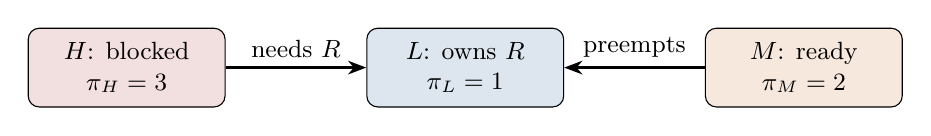
\begin{tikzpicture}[font=\small,box/.style={draw,rounded corners,align=center,minimum width=2.5cm,minimum height=1cm}]
    \node[box,fill=osred!15] (high) at (0,0) {$H$: blocked\\$\pi_H=3$};
    \node[box,fill=osblue!15] (low) at (4.3,0) {$L$: owns $R$\\$\pi_L=1$};
    \node[box,fill=osorange!15] (medium) at (8.6,0) {$M$: ready\\$\pi_M=2$};
    \draw[-{Stealth},thick] (high)--node[above]{needs $R$}(low);
    \draw[-{Stealth},thick] (medium)--node[above]{preempts}(low);
  \end{tikzpicture}
  \end{center}
  \begin{block}{Decompose the blocked interval}
    $B_H=$ remaining owner execution $+$ intervening execution $+$ suspension/overhead. PIP targets unrelated medium-priority interference, not every term.
  \end{block}
  \smallnote{CPU aging cannot make a mutex available. Accelerate the dependency's owner, not just the blocked requester.}
\end{frame}

\begin{frame}{Priority inheritance protocol (PIP)}
  \small When $H$ blocks on a mutex owned by $L$:
  \begin{enumerate}
    \item raise $L$ to the highest effective priority among its blocked waiters;
    \item propagate donation through nested lock dependencies;
    \item recompute effective priority as waiters and owned locks change.
  \end{enumerate}
  \[
    \pi_i^{\mathrm{eff}}=\max\!\left(\pi_i^{\mathrm{base}},
      \max_{j\in\mathcal{W}(i)}\pi_j^{\mathrm{eff}}\right),
  \]
  where $\mathcal{W}(i)$ contains waiters on all PI-enabled mutexes held by $i$; omit the inner maximum if empty.
  \begin{alertblock}{Inheritance changes rank, not ownership or readiness}
    $H$ remains blocked. A runnable owner outranks unrelated medium-priority work, but still-higher work can interfere. Basic PIP does not prevent deadlock or all chained blocking.
  \end{alertblock}
  \note{The formula is recursive: donate effective rather than just base priority. Mutex release, waiter timeout, and cancellation can change the maximum. Linux rt-mutex documentation describes both boosting and deboosting through chains.}
\end{frame}

\begin{frame}{PIP example 1: measure inversion before and after}
  \small Jobs $(a,b,\pi)$: $L=(0,3,1)$, $M=(1,8,2)$, $H=(1,1,3)$.
  $L$ holds $R$ throughout its 3 CPU units; $H$ requests $R$ on arrival.
  Lock operations and switches cost zero; $M$ never uses $R$.
  \begin{center}
  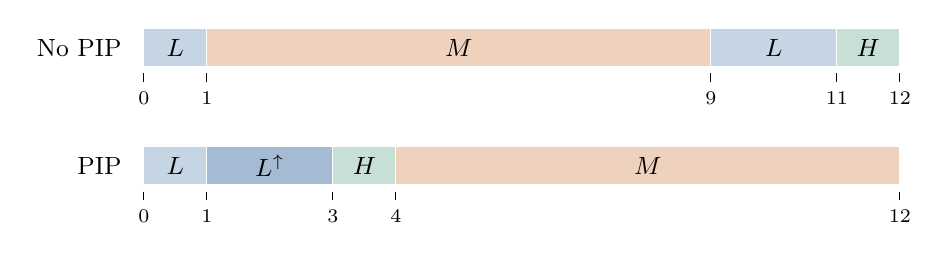
\begin{tikzpicture}[x=.8cm,y=.7cm,font=\small]
    \node[anchor=east] at (-.2,.55) {No PIP};
    \runblock{0}{1}{$L$}{osblue!25}
    \runblock{1}{9}{$M$}{osorange!30}
    \runblock{9}{11}{$L$}{osblue!25}
    \runblock{11}{12}{$H$}{osgreen!25}
    \runticks{0,1,9,11,12}
    \begin{scope}[yshift=-1.5cm]
      \node[anchor=east] at (-.2,.55) {PIP};
      \runblock{0}{1}{$L$}{osblue!25}
      \runblock{1}{3}{$L^{\uparrow}$}{osblue!40}
      \runblock{3}{4}{$H$}{osgreen!25}
      \runblock{4}{12}{$M$}{osorange!30}
      \runticks{0,1,3,4,12}
    \end{scope}
  \end{tikzpicture}
  \end{center}
  \[B_H^{\mathrm{no\ PIP}}=11-1=10=2+8,\qquad B_H^{\mathrm{PIP}}=3-1=2.\]
  \smallnote{$L^{\uparrow}$ inherits $H$'s priority; $H$ stays blocked until $R$ is released.}
\end{frame}

\begin{frame}{PIP example 2: transitive donation across two locks}
  \small Snapshot: $\pi_H=9$, $\pi_M=5$, $\pi_L=2$, $\pi_K=1$.
  $H$ waits on $R_1$ owned by $L$; $L$ waits on $R_2$ owned by $K$.
  $M$ is independent and ready; no other tasks, arrivals, or overhead.
  \begin{center}
  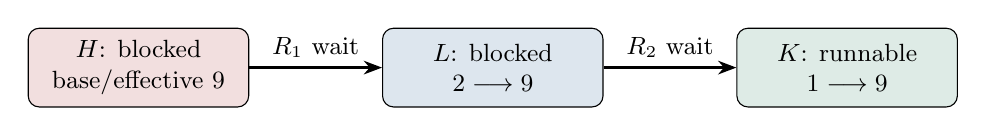
\begin{tikzpicture}[font=\small,box/.style={draw,rounded corners,align=center,minimum width=2.8cm,minimum height=1cm}]
    \node[box,fill=osred!15] (high) at (0,0) {$H$: blocked\\base/effective $9$};
    \node[box,fill=osblue!15] (low) at (4.5,0) {$L$: blocked\\$2\longrightarrow9$};
    \node[box,fill=osgreen!15] (owner) at (9,0) {$K$: runnable\\$1\longrightarrow9$};
    \draw[-{Stealth},thick] (high)--node[above]{$R_1$ wait}(low);
    \draw[-{Stealth},thick] (low)--node[above]{$R_2$ wait}(owner);
  \end{tikzpicture}
  \end{center}
  If $K$ needs 2 CPU units to release $R_2$ and then $L$ needs 1 to release $R_1$, $H$'s remaining blocking is $2+1=3$ units with PIP.
  \begin{alertblock}{Correct restoration is also transitive}
    Recompute from all held locks and remaining waiters after unlock, timeout, or cancellation. Do not blindly reset to base priority.
  \end{alertblock}
  \note{K runs despite M. After R2 is released, L inherits 9 via H and finishes R1. No self-suspension is allowed in the three-unit bound. Cyclic dependencies still deadlock under basic PIP.}
\end{frame}

\begin{frame}{Priority ceilings: specify which protocol}
  \small Resource ceiling: $\Pi(R)=\max\{\pi_i:i\text{ may lock }R\}$.
  \begin{columns}[T,onlytextwidth]
    \column{.48\textwidth}
    \begin{block}{Original ceiling protocol}
      A free lock can be acquired only if the requester's effective rank exceeds all ceilings of locks held by \emph{other} tasks. Inherit priority when this rule blocks a requester.
    \end{block}
    \column{.48\textwidth}
    \begin{block}{Immediate ceiling protocol}
      At acquisition, immediately raise the owner's effective rank to at least the resource ceiling, even without a waiting high-priority task.
    \end{block}
  \end{columns}
  \begin{itemize}
    \item Classical guarantees assume one CPU, fixed base ranks, correct ceilings, nested locks, no equal-rank preemption, and no suspension while holding locks.
    \item These assumptions are stronger than ``use a high-priority mutex.''
  \end{itemize}
  \note{The original and immediate protocols have different admission mechanisms. Under their classical uniprocessor assumptions they prevent lock deadlock and bound lower-priority blocking by one relevant critical section. See Sha, Rajkumar, and Lehoczky (1990).}
\end{frame}

\begin{frame}{Deriving a ceiling-based blocking bound}
  \small Under the classical ceiling-protocol assumptions, $C_{k,R}^{\mathrm{cs}}$ bounds the CPU duration of a lower-priority task's critical section:
  \[
    B_i\le\max\left(\{0\}\cup
      \{C_{k,R}^{\mathrm{cs}}:\pi_k<\pi_i,\ \Pi(R)\ge\pi_i\}\right).
  \]
  \begin{block}{Example: filter the resources before taking a maximum}
    Target $\pi_i=4$. A lower-priority task uses $R_A$ with ceiling 5 for 2 ms; another uses $R_B$ with ceiling 3 for 7 ms. Only $R_A$ qualifies: $B_i\le2$ ms, not 7 ms and not 9 ms.
  \end{block}
  \begin{itemize}
    \item Include nested execution in the enclosing critical-section duration.
    \item Add higher-priority interference separately in response-time analysis.
    \item Basic PIP need not yield this single-section maximum: multiple blocking episodes can occur.
  \end{itemize}
\end{frame}

\begin{frame}{Choose the remedy for the actual dependency}
  \small\renewcommand{\arraystretch}{1.2}
  \begin{tabularx}{\textwidth}{@{}lLL@{}}
    \toprule
    \textbf{Mechanism} & \textbf{Helps with} & \textbf{Does not automatically solve} \\
    \midrule
    Aging / global boost & low-priority ready waiting & unavailable locks or I/O \\
    PIP & medium-priority interference & cycles, suspension, overload \\
    Ceiling protocol & bounded lower-priority blocking & arbitrary multicore locking \\
    Global lock order & circular-wait deadlock & inversion or unfair service \\
    Shorter / split locks & serialization and convoys & every fairness requirement \\
    Admission / backpressure & excessive offered work & correctness of lock acquisition \\
    \bottomrule
  \end{tabularx}
  \smallnote{Timeouts need rollback or cancellation semantics. Blind retries can turn deadlock into livelock rather than useful progress.}
\end{frame}


\section{Multilevel Queue Scheduling}
% =============================================================================

\begin{frame}{Multilevel queue (MLQ): static classification}
  \begin{block}{Definition}
    Runnable entities are permanently assigned to classes/queues. Each queue has an internal policy, and a separate policy allocates CPU time among queues.
  \end{block}
  \begin{center}
    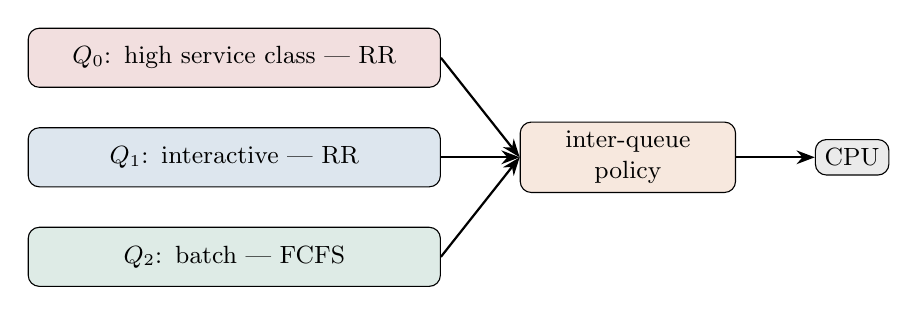
\begin{tikzpicture}[node distance=5mm,font=\small,
      q/.style={draw,rounded corners,text width=5cm,align=center,minimum height=.75cm},
      a/.style={-{Stealth},thick}]
      \node[q,fill=osred!15] (q0) {$Q_0$: high service class --- RR};
      \node[q,fill=osblue!15,below=of q0] (q1) {$Q_1$: interactive --- RR};
      \node[q,fill=osgreen!15,below=of q1] (q2) {$Q_2$: batch --- FCFS};
      \node[draw,rounded corners,text width=2.5cm,align=center,right=1cm of q1,fill=osorange!15] (arb) {inter-queue\\policy};
      \node[draw,rounded corners,right=1cm of arb,fill=black!8] (cpu) {CPU};
      \draw[a] (q0.east)--(arb.west); \draw[a] (q1.east)--(arb.west); \draw[a] (q2.east)--(arb.west);
      \draw[a] (arb)--(cpu);
    \end{tikzpicture}
  \end{center}
  \smallnote{Static classification is useful when classes have genuine semantic differences, not merely inferred behavior.}
\end{frame}

\begin{frame}{Two independent policy layers}
  \begin{columns}[T,onlytextwidth]
    \column{0.49\textwidth}
      \begin{block}{Within each queue}
        \begin{itemize}
          \item FIFO, RR, priority, or deadline;
          \item queue-specific quantum;
          \item class-specific admission control.
        \end{itemize}
      \end{block}
    \column{0.47\textwidth}
      \begin{block}{Between queues}
        \begin{itemize}
          \item strict fixed priority;
          \item weighted time shares;
          \item reservations or bandwidth caps;
          \item hierarchical fair sharing.
        \end{itemize}
      \end{block}
  \end{columns}
  \begin{alertblock}{Common mistake}
    Saying ``MLQ uses RR'' is incomplete. RR may govern one queue, while another policy decides when that queue runs at all.
  \end{alertblock}
\end{frame}

\begin{frame}{Example conventions: state the entire queue policy}
  \small All following MLQ/MLFQ examples use one CPU, one burst per job, no I/O, zero overhead, and time starting at 0. Intervals are $[s,e)$.
  \[
    T_i=c_i-a_i,\qquad W_i=T_i-b_i,\qquad R_i=s_i-a_i.
  \]
  $s_i$ is first start and $c_i$ completion. Report time-unit means; $R_i$ here is first-service delay, not the later real-time response bound.
  \begin{block}{Strict MLQ examples}
    $Q_0$ outranks $Q_1$, which outranks $Q_2$ if present. Higher-queue arrivals preempt; equal-queue arrivals do not. Preserve a preempted job's unused slice and place it at its queue's front.
  \end{block}
  \begin{itemize}
    \item Process completion before any requeue; an exhausted job leaves the system.
    \item Enqueue arrivals before quantum-expired jobs; simultaneous arrivals use alphabetical order.
    \item Queue membership is fixed for MLQ. Labels $A_k$ mean job $A$ executes in $Q_k$.
  \end{itemize}
\end{frame}

\begin{frame}{Strict MLQ example 1: three jobs in two queues}
  \small Workload $(a,b,Q)$: $A=(0,4,Q_1)$, $B=(1,3,Q_0)$, $C=(2,1,Q_0)$.
  $Q_0$: RR with $q=2$; $Q_1$: FCFS. Strict inter-queue priority; zero overhead.
  \begin{center}
  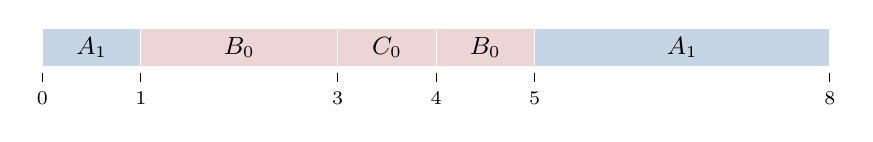
\begin{tikzpicture}[x=1.25cm,y=.7cm,font=\small]
    \runblock{0}{1}{$A_1$}{osblue!25}
    \runblock{1}{3}{$B_0$}{osred!20}
    \runblock{3}{4}{$C_0$}{osred!20}
    \runblock{4}{5}{$B_0$}{osred!20}
    \runblock{5}{8}{$A_1$}{osblue!25}
    \runticks{0,1,3,4,5,8}
  \end{tikzpicture}
  \end{center}
  \renewcommand{\arraystretch}{1.1}
  \begin{tabularx}{\textwidth}{@{}*{5}{C}@{}}
    \toprule
    \textbf{Job} & $c_i$ & $T_i$ & $W_i$ & $R_i$ \\
    \midrule
    $A$ & 8 & 8 & 4 & 0 \\
    $B$ & 5 & 4 & 1 & 0 \\
    $C$ & 4 & 2 & 1 & 1 \\
    \midrule
    Mean & & 4.67 & 2.00 & 0.33 \\
    \bottomrule
  \end{tabularx}
  \smallnote{FCFS within $Q_1$ does not prevent preemption by $Q_0$. $C$ waits for $B$'s slice to end.}
\end{frame}

\begin{frame}{Strict MLQ example 2: six jobs and three queues}
  \small Workload $(a,b,Q)$:
  \[
    \begin{gathered}
      A=(0,6,Q_2),\ B=(0,4,Q_1),\ C=(2,3,Q_0),\\
      D=(3,2,Q_0),\ E=(6,2,Q_1),\ F=(8,1,Q_0).
    \end{gathered}
  \]
  $Q_0$: RR $q=2$; $Q_1$: RR $q=3$; $Q_2$: FCFS. Strict queue priority; preserve slices across higher-queue interruptions; zero overhead.
  \begin{center}
  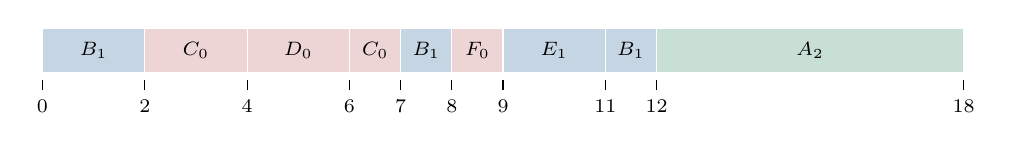
\begin{tikzpicture}[x=.65cm,y=.8cm,font=\scriptsize]
    \runblock{0}{2}{$B_1$}{osblue!25}
    \runblock{2}{4}{$C_0$}{osred!20}
    \runblock{4}{6}{$D_0$}{osred!20}
    \runblock{6}{7}{$C_0$}{osred!20}
    \runblock{7}{8}{$B_1$}{osblue!25}
    \runblock{8}{9}{$F_0$}{osred!20}
    \runblock{9}{11}{$E_1$}{osblue!25}
    \runblock{11}{12}{$B_1$}{osblue!25}
    \runblock{12}{18}{$A_2$}{osgreen!25}
    \runticks{0,2,4,6,7,8,9,11,12,18}
  \end{tikzpicture}
  \end{center}
  \meanresults{7.33}{4.33}{2.67}
  \note{B uses two units at 0--2 and its last slice unit at 7--8. At time 8 its slice expires as F arrives; B joins behind E in Q1. After F finishes, E precedes B. A first runs at time 12, illustrating inter-queue delay.}
\end{frame}

\begin{frame}{Strict priority versus weighted service}
  \small
  \begin{tabularx}{\textwidth}{@{}lXX@{}}
    \toprule
    & \textbf{Strict inter-queue priority} & \textbf{Weighted allocation} \\
    \midrule
    rule & serve highest nonempty queue & give queue $k$ a configured share $w_k/\sum_jw_j$ \\
    strength & low latency for high class & protects lower-class bandwidth \\
    failure mode & lower queues may starve & latency depends on allocation period and burstiness \\
    suitable for & truly dominant critical class & tenants, users, service groups \\
    \bottomrule
  \end{tabularx}
  \begin{tcolorbox}[title=Unused capacity,colback=osgreen!5,colframe=osgreen!70]
    A work-conserving weighted scheduler redistributes unused capacity among active queues. State whether unused credit is discarded or carried forward; weights alone do not specify that rule.
  \end{tcolorbox}
\end{frame}

\begin{frame}{Weighted MLQ: one explicit cyclic-budget policy}
  \small Two fixed queues, FCFS within each. Repeatedly visit $Q_0$ for up to 3 CPU units, then $Q_1$ for up to 1 unit. Start in $Q_0$ at $t=0$.
  \begin{itemize}
    \item A budget belongs to the queue, not one job; a completion passes residual budget to the next FCFS job there.
    \item On budget expiry, switch queues; an unfinished job retains the head position.
    \item If a queue empties, forfeit its residual budget and immediately visit the other. Empty visits consume no time; there is no banked credit.
    \item Arrivals do not interrupt an active visit; enqueue them before selection at a boundary.
  \end{itemize}
  \[
    \text{with both queues backlogged:}\qquad
    \rho_0=\frac{3}{4},\quad\rho_1=\frac{1}{4}.
  \]
  \smallnote{This is a pedagogical weighted-MLQ variant, not an implementation claim about Linux. Short finite workloads need not receive the long-run 3:1 ratio.}
\end{frame}

\begin{frame}{Weighted MLQ example 1: shared queue budgets}
  \small Workload $(a,b,Q)$: $A=(0,5,Q_0)$, $B=(0,3,Q_1)$, $C=(2,1,Q_0)$.
  Cyclic budgets $(3,1)$; FCFS within queues; start $Q_0$; zero overhead.
  \begin{center}
  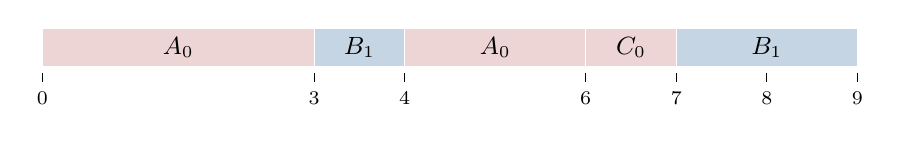
\begin{tikzpicture}[x=1.15cm,y=.7cm,font=\small]
    \runblock{0}{3}{$A_0$}{osred!20}
    \runblock{3}{4}{$B_1$}{osblue!25}
    \runblock{4}{6}{$A_0$}{osred!20}
    \runblock{6}{7}{$C_0$}{osred!20}
    \runblock{7}{9}{$B_1$}{osblue!25}
    \runticks{0,3,4,6,7,8,9}
  \end{tikzpicture}
  \end{center}
  \renewcommand{\arraystretch}{1.1}
  \begin{tabularx}{\textwidth}{@{}*{5}{C}@{}}
    \toprule
    \textbf{Job} & $c_i$ & $T_i$ & $W_i$ & $R_i$ \\
    \midrule
    $A$ & 6 & 6 & 1 & 0 \\
    $B$ & 9 & 9 & 6 & 3 \\
    $C$ & 7 & 5 & 4 & 4 \\
    \midrule
    Mean & & 6.67 & 3.67 & 2.33 \\
    \bottomrule
  \end{tabularx}
  \smallnote{At $t=6$, $C$ uses $Q_0$'s remaining budget. At $t=8$, an empty $Q_0$ is skipped, so $B$ continues.}
\end{frame}

\begin{frame}{Weighted MLQ example 2: six jobs and unused capacity}
  \small Workload $(a,b,Q)$:
  \[
    \begin{gathered}
      A=(0,6,Q_0),\ B=(0,4,Q_1),\ C=(2,3,Q_0),\\
      D=(4,2,Q_1),\ E=(6,2,Q_0),\ F=(9,1,Q_1).
    \end{gathered}
  \]
  Cyclic budgets $(3,1)$; FCFS within queues; start $Q_0$; discard unused visit budget, skip empty queues; zero overhead.
  \begin{center}
  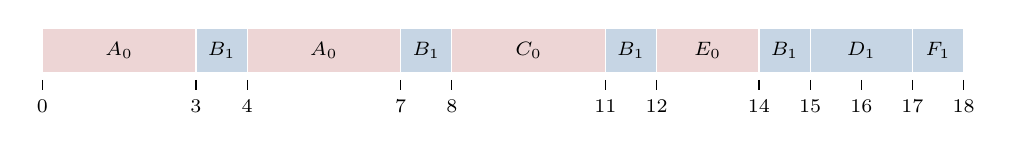
\begin{tikzpicture}[x=.65cm,y=.8cm,font=\scriptsize]
    \runblock{0}{3}{$A_0$}{osred!20}
    \runblock{3}{4}{$B_1$}{osblue!25}
    \runblock{4}{7}{$A_0$}{osred!20}
    \runblock{7}{8}{$B_1$}{osblue!25}
    \runblock{8}{11}{$C_0$}{osred!20}
    \runblock{11}{12}{$B_1$}{osblue!25}
    \runblock{12}{14}{$E_0$}{osred!20}
    \runblock{14}{15}{$B_1$}{osblue!25}
    \runblock{15}{17}{$D_1$}{osblue!25}
    \runblock{17}{18}{$F_1$}{osblue!25}
    \runticks{0,3,4,7,8,11,12,14,15,16,17,18}
  \end{tikzpicture}
  \end{center}
  \meanresults{10.17}{7.17}{5.67}
  \note{Q0 empties at 14 after consuming only two units of its visit. Its last unit is discarded. Q1 then drains without idle gaps; ticks at 15 and 16 still mark budget boundaries even if the same queue or job continues.}
\end{frame}

\begin{frame}{Hierarchical scheduling expresses organizational policy}
  \begin{center}
    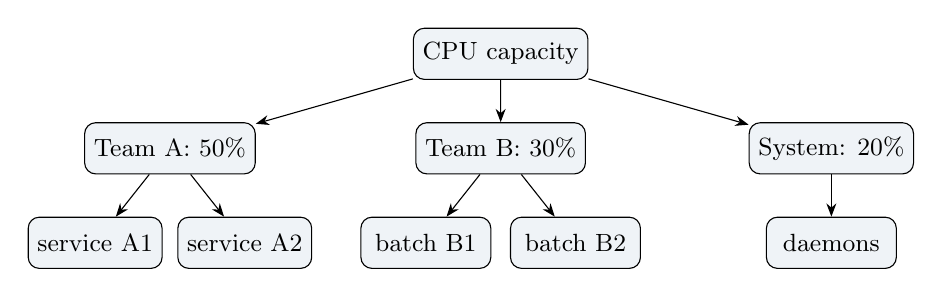
\begin{tikzpicture}[level distance=1.2cm,font=\small,
      level 1/.style={sibling distance=4.2cm},
      level 2/.style={sibling distance=1.9cm},
      every node/.style={draw,rounded corners,fill=osblue!7,minimum width=1.65cm,minimum height=.65cm},
      edge from parent/.style={draw,-{Stealth}}]
      \node {CPU capacity}
        child {node {Team A: 50\%}
          child {node {service A1}}
          child {node {service A2}}}
        child {node {Team B: 30\%}
          child {node {batch B1}}
          child {node {batch B2}}}
        child {node {System: 20\%}
          child {node {daemons}}};
    \end{tikzpicture}
  \end{center}
  \begin{itemize}
    \item First divide capacity among groups; then schedule tasks inside each group.
    \item This prevents a user with many runnable threads from automatically receiving a larger organizational share.
  \end{itemize}
\end{frame}

% =============================================================================
\section{Multilevel Feedback Queue Scheduling}
% =============================================================================

\begin{frame}{MLFQ: infer behavior from observed execution}
  \begin{block}{Core idea}
    MLFQ dynamically changes queue level using recent CPU consumption and waiting history, approximating short-job preference without knowing future bursts.
  \end{block}
  \begin{itemize}
    \item New jobs enter the highest queue; behavior can preserve or change their level. Short latency depends on competing work.
    \item Tasks that repeatedly consume full allotments move downward.
    \item Lower queues use longer quanta, reducing overhead for CPU-bound work.
    \item Periodic boosts or aging restore opportunity and adapt to phase changes.
  \end{itemize}
  \begin{alertblock}{MLFQ is a design family, not one algorithm}
    Queue count, quanta, allotments, boost interval, I/O accounting, and tie rules must all be specified.
  \end{alertblock}
\end{frame}

\begin{frame}{A complete reference rule set}
  One pedagogical MLFQ can be defined by:
  \begin{enumerate}
    \item run the highest nonempty queue; preempt when a higher queue becomes ready;
    \item use RR within each queue;
    \item admit new jobs to $Q_0$;
    \item charge all CPU time at a level against an \emph{allotment}, even across early yields;
    \item demote after the allotment is exhausted; and
    \item every $B$ time units, boost all runnable jobs, including the running job, to $Q_0$ and reset their quantum/allotment budgets.
  \end{enumerate}
  \begin{tcolorbox}[title=Why allotment rather than one uninterrupted quantum?,colback=osorange!5,colframe=osorange!70]
    Accumulated accounting prevents a CPU-bound task from avoiding demotion by yielding just before each timer interrupt.
  \end{tcolorbox}
  \note{Some historical formulations preserved priority after an early I/O yield. Present that as a parameter, not a universal MLFQ rule; it is susceptible to gaming unless CPU use is accumulated.}
\end{frame}

\begin{frame}{MLFQ accounting: three quantities, not one timer}
  \small For each job maintain remaining service $r_i$, remaining slice $s_i$, and remaining level allotment $a_i^{\mathrm{level}}$.
  \[
    (r_i,s_i,a_i^{\mathrm{level}})\leftarrow
    (r_i-d,s_i-d,a_i^{\mathrm{level}}-d)
    \quad\text{after }d\text{ CPU units}.
  \]
  \begin{itemize}
    \item $r_i=0$: finish, even if the quantum or allotment also expires.
    \item Allotment exhausted: demote, initialize the next level's budgets.
    \item Slice exhausted only: requeue at the same level with a fresh slice.
    \item Higher-level preemption: preserve both budgets; resume from the front of the interrupted queue. Equal-level arrivals do not preempt.
    \item At the bottom level, use RR with no further demotion.
  \end{itemize}
  \smallnote{$a_i^{\mathrm{level}}$ is a budget, not arrival time $a_i$. Both examples explicitly specify whether an allotment spans one or two quanta.}
\end{frame}

\begin{frame}{MLFQ event order makes the trace reproducible}
  \small At a shared event time $t$:
  \begin{enumerate}
    \item Charge elapsed CPU service; remove a completed job first.
    \item Determine any demotion or expired-slice requeue, but hold that enqueue temporarily.
    \item Enqueue arrivals at $Q_0$ in alphabetical order; then append the expired/demoted job to its resulting queue.
    \item If $t$ is a boost time, gather all unfinished runnable jobs, including the current one, order by original arrival then name, and reset them into $Q_0$.
    \item Apply higher-queue preemption if needed, then select the highest queue's head.
  \end{enumerate}
  \begin{alertblock}{This is one fully specified teaching policy}
    Other merge orders are possible. Our finite examples have no I/O; with blocking, separately specify wake-up placement, preserved usage, and how missed boosts are applied.
  \end{alertblock}
\end{frame}

\begin{frame}{MLFQ structure and feedback}
  \centering
  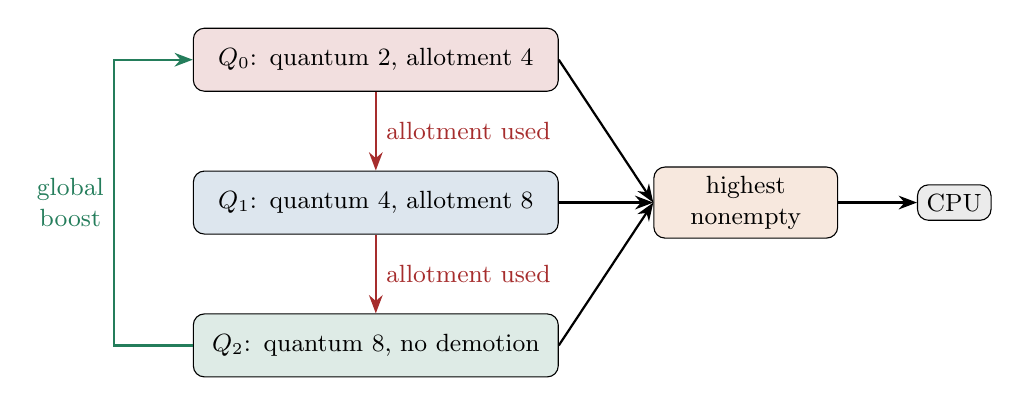
\begin{tikzpicture}[font=\small,node distance=1cm,
    q/.style={draw,rounded corners,text width=4.4cm,align=center,minimum height=.8cm},
    a/.style={-{Stealth},thick}]
    \node[q,fill=osred!15] (q0) {$Q_0$: quantum 2, allotment 4};
    \node[q,fill=osblue!15,below=of q0] (q1) {$Q_1$: quantum 4, allotment 8};
    \node[q,fill=osgreen!15,below=of q1] (q2) {$Q_2$: quantum 8, no demotion};
    \draw[a,osred] (q0.south)--node[right]{allotment used} (q1.north);
    \draw[a,osred] (q1.south)--node[right]{allotment used} (q2.north);
    \draw[a,osgreen] (q2.west)--++(-1,0) |- node[pos=.25,left,align=center]{global\\boost} (q0.west);
    \node[draw,rounded corners,text width=2.1cm,align=center,right=1.2cm of q1,fill=osorange!15] (pick) {highest\\nonempty};
    \node[draw,rounded corners,right=1cm of pick,fill=black!8] (cpu) {CPU};
    \draw[a] (q0.east)--(pick.west); \draw[a] (q1.east)--(pick.west); \draw[a] (q2.east)--(pick.west);
    \draw[a] (pick)--(cpu);
  \end{tikzpicture}
\end{frame}
% Small MLFQ trace, with per-job verification metrics.
\begin{frame}{MLFQ example 1: three jobs and preserved usage}
  \small Workload $(a,b)$: $A=(0,12)$, $B=(3,1)$, $C=(6,2)$.
  Quanta $(2,4,8)$; allotments $(2,4,\infty)$; no boosts. All enter $Q_0$; preserve slice/allotment on higher-queue preemption; zero overhead.
  \begin{center}
  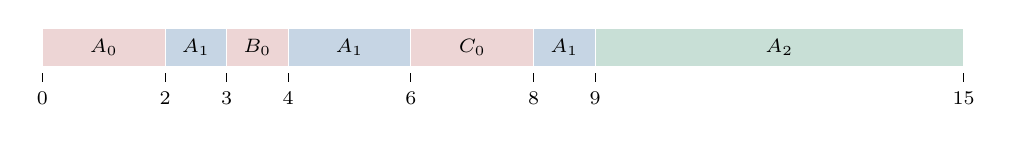
\begin{tikzpicture}[x=.78cm,y=.7cm,font=\scriptsize]
    \runblock{0}{2}{$A_0$}{osred!20}
    \runblock{2}{3}{$A_1$}{osblue!25}
    \runblock{3}{4}{$B_0$}{osred!20}
    \runblock{4}{6}{$A_1$}{osblue!25}
    \runblock{6}{8}{$C_0$}{osred!20}
    \runblock{8}{9}{$A_1$}{osblue!25}
    \runblock{9}{15}{$A_2$}{osgreen!25}
    \runticks{0,2,3,4,6,8,9,15}
  \end{tikzpicture}
  \end{center}
  \renewcommand{\arraystretch}{1.1}
  \begin{tabularx}{\textwidth}{@{}*{5}{C}@{}}
    \toprule
    \textbf{Job} & $c_i$ & $T_i$ & $W_i$ & $R_i$ \\
    \midrule
    $A$ & 15 & 15 & 3 & 0 \\
    $B$ & 4 & 1 & 0 & 0 \\
    $C$ & 8 & 2 & 0 & 0 \\
    \midrule
    Mean & & 6.00 & 1.00 & 0.00 \\
    \bottomrule
  \end{tabularx}
  \smallnote{$A$ consumes $1+2+1=4$ units in $Q_1$ across interruptions, so it demotes at $t=9$, not after a fresh four-unit slice.}
\end{frame}

\begin{frame}{MLFQ example 2: six jobs, two-quanta allotments, and a boost}
  \small Workload $(a,b)$:
  $A=(0,14)$, $B=(1,6)$, $C=(4,1)$, $D=(6,5)$, $E=(11,2)$, $F=(14,3)$.
  Quanta $(2,4,8)$; allotments $(4,8,\infty)$; boost every 16 units; zero overhead.
  \begin{center}
  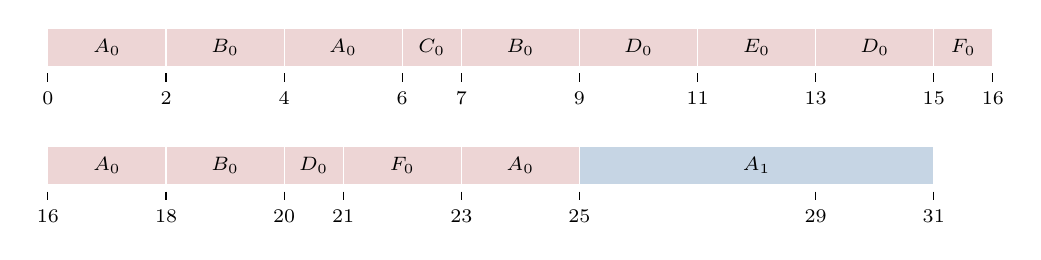
\begin{tikzpicture}[x=.75cm,y=.7cm,font=\scriptsize]
    \runblock{0}{2}{$A_0$}{osred!20}
    \runblock{2}{4}{$B_0$}{osred!20}
    \runblock{4}{6}{$A_0$}{osred!20}
    \runblock{6}{7}{$C_0$}{osred!20}
    \runblock{7}{9}{$B_0$}{osred!20}
    \runblock{9}{11}{$D_0$}{osred!20}
    \runblock{11}{13}{$E_0$}{osred!20}
    \runblock{13}{15}{$D_0$}{osred!20}
    \runblock{15}{16}{$F_0$}{osred!20}
    \runticks{0,2,4,6,7,9,11,13,15,16}
    \begin{scope}[yshift=-1.5cm,xshift=-12cm]
      \runblock{16}{18}{$A_0$}{osred!20}
      \runblock{18}{20}{$B_0$}{osred!20}
      \runblock{20}{21}{$D_0$}{osred!20}
      \runblock{21}{23}{$F_0$}{osred!20}
      \runblock{23}{25}{$A_0$}{osred!20}
      \runblock{25}{31}{$A_1$}{osblue!25}
      \runticks{16,18,20,21,23,25,29,31}
    \end{scope}
  \end{tikzpicture}
  \end{center}
  \smallnote{Two rows continue one timeline. At $t=16$, boost order is $A,B,D,F$ with remaining service $10,2,1,2$; all budgets reset, including running $F$'s. Subscript = queue.}
  \meanresults{13.17}{8.00}{1.17}
  \note{At time 4, C enqueues before expired B, but previously waiting A still runs first. A and B exhaust their top allotments at 6 and 9; D at 15. F is interrupted by the time-16 boost. At 29 A renews its Q1 quantum without demotion because it has used only four of eight allotted units there.}
\end{frame}


\begin{frame}{Response and throughput trade-offs in MLFQ}
  \begin{columns}[T,onlytextwidth]
    \column{0.49\textwidth}
      \textbf{Short upper-level quanta}
      \begin{itemize}
        \item improve response to new tasks;
        \item increase timer/context-switch cost;
        \item may disrupt cache locality.
      \end{itemize}
    \column{0.47\textwidth}
      \textbf{Long lower-level quanta}
      \begin{itemize}
        \item amortize dispatch overhead;
        \item favor throughput and locality;
        \item raise latency if boosts are too rare.
      \end{itemize}
  \end{columns}
  \begin{tcolorbox}[title=Parameter interaction,colback=ospurple!5,colframe=ospurple!65]
    Queue quanta cannot be tuned independently of allotments, boost interval, arrival rate, and context-switch cost.
  \end{tcolorbox}
\end{frame}

\begin{frame}{Gaming, phase changes, and periodic boosts}
  \begin{itemize}
    \item \textbf{Gaming:} a task yields before its quantum expires to retain high priority.
    \item \textbf{Countermeasure:} charge cumulative CPU usage per level, not only uninterrupted bursts.
    \item \textbf{Phase change:} a formerly CPU-bound task becomes interactive but remains in a low queue.
    \item \textbf{Countermeasure:} periodic global boost or wait-time promotion.
    \item \textbf{Boost too often:} CPU-bound jobs repeatedly regain top priority.
    \item \textbf{Boost too rarely:} lower-level response becomes poor and starvation-like.
  \end{itemize}
  \begin{alertblock}{Security perspective}
    Any behavior-based policy is an incentive system. Ask how an adversarial or merely unusual workload can manipulate its signals.
  \end{alertblock}
\end{frame}

\begin{frame}{MLQ versus MLFQ}
  \small
  \begin{tabularx}{\textwidth}{@{}lXX@{}}
    \toprule
    & \textbf{MLQ} & \textbf{MLFQ} \\
    \midrule
    queue membership & static semantic class & dynamic behavioral estimate \\
    movement & normally none & demotion/promotion/boost \\
    primary use & isolation among known classes & responsiveness without burst knowledge \\
    starvation & possible under strict inter-queue priority & possible if boost/aging is absent or inadequate \\
    predictability & clearer class contract & workload- and parameter-dependent \\
    gaming surface & class assignment & yield/usage patterns \\
    \bottomrule
  \end{tabularx}
\end{frame}

% =============================================================================
\section{Real-Time Priority Analysis}
% =============================================================================

\begin{frame}{Priority is not the same as a deadline guarantee}
  A high priority expresses ordering; a guarantee requires a workload model and schedulability analysis.
  \begin{itemize}
    \item Periodic/sporadic task $\tau_i=(C_i,T_i,D_i)$: worst-case execution $C_i$, period/minimum interarrival $T_i$, relative deadline $D_i$.
    \item Fixed-priority preemptive scheduling often assigns priority by period or deadline.
    \item Blocking, release jitter, interrupts, and overhead must be included for credible guarantees.
  \end{itemize}
  \begin{alertblock}{General-purpose ``real-time priority'' is dangerous}
    A runaway highest-priority thread can prevent essential lower-priority system work. Privilege, admission control, watchdogs, and budgets matter.
  \end{alertblock}
\end{frame}

\begin{frame}{Fixed-priority response-time analysis}
  \small One preemptive CPU; sporadic tasks with constrained deadlines $D_i\le T_i$; fixed priorities; valid blocking bounds; no release jitter, self-suspension, or overhead:
  \[
    R_i^{(k+1)} = C_i + B_i
      + \sum_{j\in hp(i)}
        \left\lceil\frac{R_i^{(k)}}{T_j}\right\rceil C_j,
  \]
  where $hp(i)$ is the set of higher-priority tasks and $B_i$ bounds lower-priority resource blocking.
  \begin{enumerate}
    \item initialize $R_i^{(0)}=C_i+B_i$;
    \item iterate until a fixed point or until $R_i>D_i$;
    \item declare the task schedulable if the fixed point satisfies $R_i\le D_i$.
  \end{enumerate}
  \begin{tcolorbox}[title=Interpretation,colback=osgreen!5,colframe=osgreen!70]
    The ceiling counts how many jobs of each higher-priority task can interfere during $\tau_i$'s response window.
  \end{tcolorbox}
  \smallnote{Here $R_i$ means release-to-completion response, not first-service delay in the finite-job examples. A converged upper bound within $D_i$ establishes schedulability.}
  \note{Interference counting uses a half-open response window, so a release exactly at completion does not add another interfering job. Blocking must be justified by the actual resource protocol. An overly conservative blocking bound can make the test pessimistic.}
\end{frame}

\begin{frame}{Response-time example 1: three tasks and one blocking term}
  \small Full task set $(C,T,D)$, in descending priority:
  $\tau_1=(1,4,4)$, $\tau_2=(2,7,7)$, $\tau_3=(1,20,20)$.
  Protocol-derived blocking bounds: $(B_1,B_2,B_3)=(0,1,0)$.
  \begin{align*}
    R_2^{(0)} &= C_2+B_2 = 3,\\
    R_2^{(1)} &= 3+\left\lceil\frac{3}{4}\right\rceil(1)=4,\\
    R_2^{(2)} &= 3+\left\lceil\frac{4}{4}\right\rceil(1)=4.
  \end{align*}
  The bound converges at $R_2=4\le D_2=7$. Also $R_1=1$, $R_3=4$; all three meet their deadlines under this model.
  \begin{alertblock}{Why include $B_2$?}
    Even a high-priority task can be delayed once by a lower-priority critical section under a bounded locking protocol.
  \end{alertblock}
\end{frame}

\begin{frame}{Response-time example 2: five tasks and repeated interference}
  \small Tasks are ordered by decreasing priority; $D_i=T_i$. Blocking bounds $B_i$ are assumed justified by the resource protocol. No jitter, suspension, or overhead.
  \par\medskip
  \renewcommand{\arraystretch}{1.1}
  \begin{tabularx}{\textwidth}{@{}*{4}{C}@{}}
    \toprule
    Task & $C_i$ & $T_i=D_i$ & $B_i$ \\
    \midrule
    $\tau_1$ & 1 & 5 & 0 \\
    $\tau_2$ & 1 & 8 & 0 \\
    $\tau_3$ & 2 & 12 & 1 \\
    $\tau_4$ & 3 & 20 & 1 \\
    $\tau_5$ & 4 & 40 & 0 \\
    \bottomrule
  \end{tabularx}
  \[
    R_5^{(k)}:4\to11\to14\to16\to17\to18\to18.
  \]
  Final bounds: $(R_1,R_2,R_3,R_4,R_5)=(1,2,5,10,18)$; every $R_i\le D_i$.
  \smallnote{Crossing an arrival threshold adds an interfering job; iterate until the bound truly stabilizes. These are response bounds, not means of a finite Gantt chart.}
\end{frame}

\begin{frame}{Rate-monotonic utilization bound: sufficient, not necessary}
  For $n$ independent periodic tasks with $D_i=T_i$, fixed priorities by shorter period, and no blocking/overhead:
  \[
    \sum_{i=1}^{n}\frac{C_i}{T_i}
      \le n\left(2^{1/n}-1\right)
  \]
  is a sufficient schedulability test.
  \begin{itemize}
    \item The bound approaches $\ln 2\approx0.693$ as $n\to\infty$.
    \item Failing the bound does \emph{not} prove failure; exact response-time analysis may still pass.
    \item Harmonic periods can schedule at much higher utilization, potentially up to 100\% under the ideal model.
  \end{itemize}
\end{frame}

% =============================================================================
\section{Modern Scheduler Architectures}
% =============================================================================

\begin{frame}{Production kernels combine scheduling classes}
  \small
  \begin{center}
    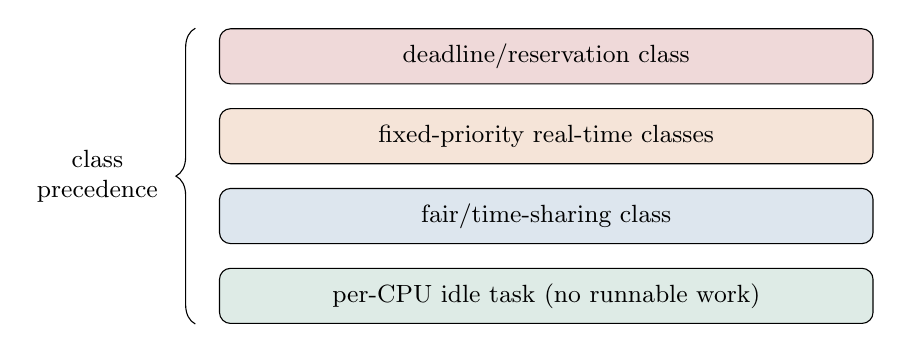
\begin{tikzpicture}[font=\small,node distance=3mm,
      q/.style={draw,rounded corners,minimum width=8.3cm,minimum height=.7cm}]
      \node[q,fill=osred!18] (dl) {deadline/reservation class};
      \node[q,fill=osorange!18,below=of dl] (rt) {fixed-priority real-time classes};
      \node[q,fill=osblue!15,below=of rt] (fair) {fair/time-sharing class};
      \node[q,fill=osgreen!15,below=of fair] (idle) {per-CPU idle task (no runnable work)};
      \draw[decorate,decoration={brace,amplitude=7pt}] ([xshift=-.3cm]idle.south west)--([xshift=-.3cm]dl.north west)
        node[midway,left=10pt,align=center]{class\\precedence};
    \end{tikzpicture}
  \end{center}
  \begin{itemize}
    \item Each class defines its own ready structures and selection rule.
    \item The kernel first selects the highest eligible class, then a task within it.
    \item Configured admission/bandwidth controls can limit high-class demand; this is not an unconditional starvation guarantee.
  \end{itemize}
  \smallnote{Conceptual ordinary Linux class ordering; special kernel/configuration paths are omitted. Background user jobs are not the per-CPU idle task.}
\end{frame}

\begin{frame}{Linux fair scheduling: from CFS toward EEVDF}
  \small
  \begin{itemize}
    \item CFS modeled weighted fair sharing using per-entity virtual runtime and historically selected the least-served entity from an ordered run queue.
    \item Current Linux fair-class development uses \concept{EEVDF}: eligible entities are ordered by virtual deadlines, combining lag-based fairness with latency requests.
    \item Nice values remain weights, not strict fixed-priority levels; higher weight means a larger long-run CPU share among competing fair tasks.
    \item Separate Linux classes handle deadline and POSIX real-time policies; cgroups add hierarchical shares and bandwidth controls.
  \end{itemize}
  \begin{tcolorbox}[title=Modern correction,colback=osorange!5,colframe=osorange!70]
    Describing Linux simply as ``CFS chooses the leftmost red-black-tree node'' is now historically useful but incomplete for the evolving fair class.
  \end{tcolorbox}
  \smallnote{Source: Linux kernel EEVDF scheduler documentation; checked September 16, 2026.}
\end{frame}

\begin{frame}{Windows: preemptive priorities with dynamic boosts}
  \begin{itemize}
    \item Windows schedules threads at priorities 0--31; a ready higher-priority thread preempts a lower-priority thread.
    \item Equal-priority ready threads receive round-robin time slices.
    \item Process priority class and thread-relative priority determine base priority.
    \item Variable-priority threads may receive temporary boosts after relevant waits; real-time-class threads require care and do not use ordinary dynamic boosts.
  \end{itemize}
  \begin{alertblock}{Priority is broader than CPU time}
    Background work can still harm responsiveness through memory, storage, and lock contention; modern systems also expose resource and quality-of-service controls.
  \end{alertblock}
  \smallnote{Source: Microsoft Learn, Scheduling Priorities; checked September 16, 2026.}
\end{frame}

\begin{frame}{Containers and groups need hierarchical control}
  Per-thread fairness alone does not isolate tenants.
  \begin{itemize}
    \item \textbf{Weight/share:} divide spare CPU proportionally among active groups.
    \item \textbf{Quota/bandwidth:} cap CPU consumption over a period.
    \item \textbf{Affinity/cpuset:} restrict eligible processors and NUMA placement.
    \item \textbf{Utilization hints:} guide placement/frequency decisions; they are not reservations of CPU time.
  \end{itemize}
  \begin{tcolorbox}[title=Containerization insight,colback=osgreen!5,colframe=osgreen!70]
    Containers do not contain a separate CPU scheduler by default; the host kernel schedules their threads under cgroup and namespace policy.
  \end{tcolorbox}
\end{frame}

\begin{frame}{Heterogeneous multicore adds a placement problem}
  Scheduling now chooses both \emph{when} and \emph{where} a task runs.
  \begin{columns}[T,onlytextwidth]
    \column{0.49\textwidth}
      \textbf{Performance concerns}
      \begin{itemize}
        \item CPU capacity and microarchitecture;
        \item cache/NUMA locality;
        \item migration and warmup cost;
        \item deadline or frame latency.
      \end{itemize}
    \column{0.47\textwidth}
      \textbf{Energy/thermal concerns}
      \begin{itemize}
        \item performance per watt;
        \item frequency-selection latency;
        \item thermal headroom;
        \item background-task caps.
      \end{itemize}
  \end{columns}
  \smallnote{A scalar priority cannot encode every objective; production schedulers combine class, weight, utilization, topology, and QoS signals.}
\end{frame}

% =============================================================================
\section{Implementation and Verification}
% =============================================================================

\begin{frame}[fragile]{Observing Linux scheduling attributes}
\begin{lstlisting}[language=bash]
# Niceness affects weight in the normal/fair class
nice -n 10 ./cpu_bound
renice 5 -p $PID

# Inspect policy, priority, affinity, and runtime fields
chrt -p $PID
taskset -pc $PID
ps -o pid,cls,rtprio,pri,ni,psr,stat,comm -p $PID

# Real-time policy changes require privilege and care
sudo chrt --fifo 20 ./short_bounded_task
\end{lstlisting}
  \begin{alertblock}{Safety}
    Never test unbounded real-time CPU loops on a production machine. Use a VM, retain a rescue shell on another CPU, and enforce a runtime limit.
  \end{alertblock}
\end{frame}

\begin{frame}[fragile]{Priority inheritance with POSIX mutexes}
\begin{lstlisting}[language=C,aboveskip=1pt,belowskip=1pt]
#include <pthread.h>
#include <stdio.h>
#include <stdlib.h>
#include <string.h>
static void check(int error) {
    if (error == 0) return;
    fprintf(stderr, "%s\n", strerror(error));
    exit(EXIT_FAILURE);
}
int main(void) {
    pthread_mutexattr_t attributes;
    pthread_mutex_t mutex;
    check(pthread_mutexattr_init(&attributes));
    check(pthread_mutexattr_setprotocol(&attributes,
                                       PTHREAD_PRIO_INHERIT));
    check(pthread_mutex_init(&mutex, &attributes));
    check(pthread_mutexattr_destroy(&attributes));
    check(pthread_mutex_destroy(&mutex));
}
\end{lstlisting}
  \smallnote{Configuration smoke test, not a contention benchmark. Build with \code{cc -std=c11 -Wall -Wextra -pthread}. Pthread functions return error numbers directly; report those, not \code{errno}.}
\end{frame}

\begin{frame}[fragile]{Event-driven queue scheduler skeleton (pseudocode)}
\begin{lstlisting}[language=Python]
while unfinished:
    expired = settle_completion_and_budgets(now)
    enqueue_arrivals(now)
    enqueue_expired_or_demoted(expired)
    apply_due_aging_or_global_boost(now)
    preserve_and_preempt_if_higher_queue_ready()
    running = retain_current_or_select_head()
    if running is None:
        now = next_arrival_time()  # record the idle interval
        continue
    event = min(next_arrival, completion, quantum_end,
                allotment_end, boost_time, aging_time)
    execute_and_charge_all_budgets(running, event - now)
    now = event
\end{lstlisting}
  \smallnote{For MLFQ, store level, remaining quantum, remaining allotment, first start, and last boost epoch explicitly.}
\end{frame}

\begin{frame}{Verification checklist}
  For every computed schedule, verify:
  \begin{enumerate}
    \item no task executes before arrival or while blocked;
    \item total executed service equals each $b_i$;
    \item the selected task is maximal under the complete policy and tie rule;
    \item preemption occurs only at defined events;
    \item priority inheritance/boosts are restored correctly;
    \item MLFQ quantum and allotment accounting remain consistent across yields; and
    \item context-switch and idle intervals are included when nonzero.
  \end{enumerate}
\end{frame}

% =============================================================================
\section{Synthesis}
% =============================================================================

\begin{frame}{Misconceptions corrected}
  \scriptsize
  \begin{tabularx}{\textwidth}{@{}XcX@{}}
    \toprule
    \textbf{Misconception} & & \textbf{Precise statement} \\
    \midrule
    Lower numeric priority always means higher urgency. & $\Rightarrow$ & Numeric convention is API/policy specific. \\
    Aging automatically prevents starvation. & $\Rightarrow$ & It needs sufficient, eventually dominant boosting and fair ties. \\
    MLFQ always promotes a task that blocks early. & $\Rightarrow$ & Promotion and accounting are design parameters. \\
    Demotion alone prevents starvation. & $\Rightarrow$ & Low queues may still starve without boosts or shares. \\
    Priority inheritance makes $H$ run immediately. & $\Rightarrow$ & It accelerates the resource owner; $H$ remains blocked. \\
    A real-time priority guarantees a deadline. & $\Rightarrow$ & Guarantees require WCET, arrival, blocking, and overhead analysis. \\
    Linux fair scheduling is just classic CFS. & $\Rightarrow$ & The fair class is transitioning to EEVDF concepts. \\
    Containers each have their own CPU scheduler. & $\Rightarrow$ & Host-kernel scheduling is shaped by cgroup policy. \\
    \bottomrule
  \end{tabularx}
\end{frame}

\begin{frame}{Policy selection by requirement}
  \small
  \begin{tabularx}{\textwidth}{@{}lXX@{}}
    \toprule
    \textbf{Requirement} & \textbf{Likely mechanism} & \textbf{Question to ask} \\
    \midrule
    critical control latency & fixed priority/deadline class & is demand admitted and blocking bounded? \\
    interactive responsiveness & feedback/latency-aware fair policy & can behavior be gamed? \\
    tenant isolation & hierarchical shares and quotas & what happens to unused capacity? \\
    background progress & aging, boosts, reserved share & is there a finite service bound? \\
    lock-dependent real time & inheritance/ceiling protocol & are critical sections bounded? \\
    mobile efficiency & topology/energy-aware placement & what latency and thermal signals are used? \\
    \bottomrule
  \end{tabularx}
\end{frame}

\begin{frame}{Key takeaways}
  \begin{itemize}
    \item Ready waiting, dependency blocking, and retry failures need different remedies.
    \item Starvation is a liveness property; aging helps only under stated assumptions.
    \item Priority inversion arises through resource ownership; inheritance and ceilings bound its effects differently.
    \item MLQ provides static class separation; MLFQ predicts behavior through feedback.
    \item MLFQ correctness depends on cumulative accounting, boosts, and fully specified parameters.
    \item Real-time guarantees require response-time or schedulability analysis, not merely high priority.
    \item Modern kernels combine scheduling classes, hierarchical controls, topology, energy, and QoS.
  \end{itemize}
\end{frame}

\begin{frame}{Next week: real-time and proportional-share scheduling}
  \begin{itemize}
    \item Rate-monotonic and deadline-monotonic priority assignment;
    \item Earliest Deadline First and processor-demand analysis;
    \item reservations, budgets, and sporadic servers;
    \item lottery and stride scheduling;
    \item overload behavior and admission control;
    \item multiprocessor real-time complications.
  \end{itemize}
  \begin{tcolorbox}[title=Preparation,colback=osgreen!5,colframe=osgreen!70]
    Review ceilings, recurrence relations, utilization, and the difference between sufficient and exact schedulability tests.
  \end{tcolorbox}
\end{frame}

% =============================================================================
\appendix
\section{Appendix}
% =============================================================================

\begin{frame}{Knowledge check: progress and dependencies}
  \begin{enumerate}
    \item Why can a mutually exclusive program still deadlock or starve?
    \item Construct a workload that indefinitely denies a runnable job service.
    \item Why does reaching the highest aging rank not by itself bound waiting?
    \item How does priority donation propagate when the owner is also blocked?
    \item Why must unlock recompute priority instead of always restoring base rank?
    \item Distinguish ordinary resource blocking from unrelated medium-priority interference.
  \end{enumerate}
\end{frame}

\begin{frame}{Exercise: preemptive priority with aging}
  Jobs $(a,b,\pi)$: $A=(0,7,1)$, $B=(1,3,3)$, $C=(2,5,2)$, $D=(3,2,4)$.
  Larger $\pi$ is higher; ties are FIFO.
  \begin{enumerate}
    \item Use Week 5's fixed-priority schedule as a baseline and record maximum wait.
    \item Specify when waiting credit resets and how equal effective ranks are ordered.
    \item Repeat with effective priority increased by one after every four units of ready waiting.
    \item State exactly when boosts occur and whether a boost can trigger immediate preemption.
    \item Compare mean latency and maximum waiting.
  \end{enumerate}
\end{frame}

\begin{frame}{Exercise: diagnose priority inversion}
  Tasks $L$, $M$, and $H$ have increasing priority. $L$ locks $R$ for 3 ms; after 1 ms, $H$ becomes ready and requests $R$; then $M$ becomes ready for 8 ms.
  \begin{enumerate}
    \item Draw the schedule without a locking protocol.
    \item Measure $H$'s direct and indirect blocking.
    \item Redraw with priority inheritance.
    \item What changes if $L$ blocks while holding $R$?
    \item Could inheritance prevent a circular-wait deadlock? Explain.
  \end{enumerate}
\end{frame}

\begin{frame}{Exercise: specify and trace an MLFQ}
  Configure $Q_0:q=2$, $Q_1:q=4$, $Q_2:q=8$, with allotments $(4,8,\infty)$ and a global boost every 20 units.
  Jobs: $A=(0,14)$, $B=(1,2)$, $C=(7,5)$.
  \begin{enumerate}
    \item State the arrival/quantum-boundary event order.
    \item Use the lecture's boost merge order and interrupted-slice preservation; draw the timeline.
    \item Track remaining service, quantum, and allotment separately.
    \item Compute response and turnaround times.
    \item Modify $A$ to yield every 1.9 units. Does cumulative accounting stop gaming?
  \end{enumerate}
\end{frame}

\begin{frame}{Exercise: response-time analysis}
  Fixed priorities follow increasing period:
  \[
    \tau_1=(C=1,T=4,D=4),\quad
    \tau_2=(1,5,5),\quad
    \tau_3=(2,10,10).
  \]
  Assume $B_1=0$, $B_2=0$, and $B_3=1$.
  \begin{enumerate}
    \item Compute utilization. Why is the plain no-blocking utilization bound insufficient here?
    \item Compute each fixed-point response time.
    \item Is every task schedulable under the model?
    \item Increase $B_3$ until its deadline is first missed.
    \item Explain why utilization alone cannot represent blocking.
  \end{enumerate}
\end{frame}

\begin{frame}{Further study}
  \begin{itemize}
    \item fixed-priority response-time analysis with jitter and self-suspension;
    \item priority inheritance, original ceiling, and immediate-ceiling protocols;
    \item BSD and historical Unix feedback schedulers;
    \item Linux EEVDF, deadline scheduling, cgroup CPU control, and utilization clamping;
    \item Windows base priorities, boosts, QoS, and heterogeneous-core placement;
    \item scheduler activations and user-level runtimes;
    \item adversarial workloads and scheduler side channels.
  \end{itemize}
  \vfill
  \begin{center}\Large Questions?\end{center}
\end{frame}

\begin{frame}{Source notes: theory and protocol contracts}
  \footnotesize
  \begin{itemize}
    \item R. and A. Arpaci-Dusseau, \emph{Operating Systems: Three Easy Pieces}, Chapter 8: MLFQ, allotment accounting, and boosts.\par
      \url{https://pages.cs.wisc.edu/~remzi/OSTEP/cpu-sched-mlfq.pdf}
    \item L. Sha, R. Rajkumar, J. P. Lehoczky (1990), \emph{Priority Inheritance Protocols: An Approach to Real-Time Synchronization}. IEEE Transactions on Computers 39(9), 1175--1185. DOI: 10.1109/12.57058.
    \item M. Joseph and P. Pandya (1986), \emph{Finding Response Times in a Real-Time System}. The Computer Journal 29(5), 390--395. DOI: 10.1093/comjnl/29.5.390.
    \item The Open Group, \code{pthread\_mutexattr\_setprotocol}: PI and ceiling attributes.\par
      \url{https://pubs.opengroup.org/onlinepubs/9799919799/}
  \end{itemize}
  \smallnote{Numerical schedules and bounds in this deck are teaching examples with explicitly stated assumptions, not production-kernel traces.}
\end{frame}

\begin{frame}{Source notes: implementation case studies}
  \footnotesize Official documentation checked September 16, 2026:
  \begin{itemize}
    \item Linux rt-mutex: inheritance, chained donation, and waiter updates.\par
      \url{https://docs.kernel.org/locking/rt-mutex.html}
    \item Linux EEVDF: eligibility/lag and virtual-deadline selection.\par
      \url{https://docs.kernel.org/scheduler/sched-eevdf.html}
    \item Linux cgroup v2: CPU weights, bandwidth limits, and resource control.\par
      \url{https://docs.kernel.org/admin-guide/cgroup-v2.html}
    \item Microsoft Learn: Scheduling Priorities.\par
      \url{https://learn.microsoft.com/en-us/windows/win32/procthread/scheduling-priorities}
  \end{itemize}
  \smallnote{Implementation behavior depends on OS version and configuration. Virtual deadlines in a fair scheduler are not application deadline guarantees.}
\end{frame}

\end{document}

